% This file was converted to LaTeX by Writer2LaTeX ver. 1.4
% see http://writer2latex.sourceforge.net for more info
\documentclass[12pt]{article}
\usepackage[utf8]{inputenc}
\usepackage[T1]{fontenc}
\usepackage[english]{babel}
\usepackage{amsmath}
\usepackage{amssymb,amsfonts,textcomp}
\usepackage{array}
\usepackage{supertabular}
\usepackage{hhline}
\usepackage{hyperref}
\hypersetup{colorlinks=true, linkcolor=blue, citecolor=blue, filecolor=blue, urlcolor=blue}
\usepackage{graphicx}
% footnotes configuration
\makeatletter
\renewcommand\thefootnote{\arabic{footnote}}
\makeatother
\newcommand\textsubscript[1]{\ensuremath{{}_{\text{#1}}}}
% Text styles
\newcommand\textstyleFootnoteSymbol[1]{{\fontsize{6.5pt}{7.8pt}\selectfont #1}}
\newcommand\textstyleListLabelxix[1]{#1}
\newcommand\textstylegd[1]{#1}
\newcommand\textstyleDatei[1]{#1}
\newcommand\textstyleInternetlink[1]{#1}
% Headings and outline numbering
\makeatletter
\renewcommand\section{\@startsection{section}{1}{0.0cm}{0.1665in}{0.0835in}{\normalfont\normalsize\fontsize{18pt}{21.6pt}\selectfont\rmfamily\bfseries\raggedright}}
\renewcommand\subsection{\@startsection{subsection}{2}{0.0cm}{0.222in}{0.0835in}{\normalfont\normalsize\fontsize{16pt}{19.2pt}\selectfont\rmfamily\bfseries\raggedright}}
\renewcommand\subsubsection{\@startsection{subsubsection}{3}{0.0cm}{0.0972in}{0.1mm}{\normalfont\normalsize\fontsize{14pt}{16.8pt}\selectfont\rmfamily\bfseries\raggedright}}
\renewcommand\@seccntformat[1]{\csname @textstyle#1\endcsname{\csname the#1\endcsname}\csname @distance#1\endcsname}
\setcounter{secnumdepth}{0}
\newcommand\@distancesection{}
\newcommand\@textstylesection[1]{#1}
\newcommand\@distancesubsection{}
\newcommand\@textstylesubsection[1]{#1}
\newcommand\@distancesubsubsection{}
\newcommand\@textstylesubsubsection[1]{#1}
\makeatother
\makeatletter
\newcommand\arraybslash{\let\\\@arraycr}
\makeatother
\raggedbottom
% Paragraph styles
\renewcommand\familydefault{\rmdefault}
\newenvironment{styleStandard}{\setlength\leftskip{0cm}\setlength\rightskip{0cm plus 1fil}\setlength\parindent{0cm}\setlength\parfillskip{0pt plus 1fil}\setlength\parskip{0in plus 1pt}\writerlistparindent\writerlistleftskip\leavevmode\normalfont\normalsize\writerlistlabel\ignorespaces}{\unskip\vspace{0.111in plus 0.0111in}\par}
\newenvironment{stylelsSectioni}{\setlength\leftskip{0.25in}\setlength\rightskip{0in plus 1fil}\setlength\parindent{0in}\setlength\parfillskip{0pt plus 1fil}\setlength\parskip{0.1665in plus 0.016649999in}\writerlistparindent\writerlistleftskip\leavevmode\normalfont\normalsize\fontsize{18pt}{21.6pt}\selectfont\bfseries\writerlistlabel\ignorespaces}{\unskip\vspace{0.0835in plus 0.00835in}\par}
\newenvironment{stylelsSectionii}{\setlength\leftskip{0.25in}\setlength\rightskip{0in plus 1fil}\setlength\parindent{0in}\setlength\parfillskip{0pt plus 1fil}\setlength\parskip{0.222in plus 0.0222in}\writerlistparindent\writerlistleftskip\leavevmode\normalfont\normalsize\fontsize{16pt}{19.2pt}\selectfont\bfseries\writerlistlabel\ignorespaces}{\unskip\vspace{0.0835in plus 0.00835in}\par}
\newenvironment{stylelsSectioniii}{\setlength\leftskip{0.5799in}\setlength\rightskip{0in plus 1fil}\setlength\parindent{-0.1299in}\setlength\parfillskip{0pt plus 1fil}\setlength\parskip{0in plus 1pt}\writerlistparindent\writerlistleftskip\leavevmode\normalfont\normalsize\fontsize{14pt}{16.8pt}\selectfont\bfseries\writerlistlabel\ignorespaces}{\unskip\vspace{0.111in plus 0.0111in}\par}
\newenvironment{styleListParagraph}{\setlength\leftskip{0.5in}\setlength\rightskip{0in plus 1fil}\setlength\parindent{0in}\setlength\parfillskip{0pt plus 1fil}\setlength\parskip{0in plus 1pt}\writerlistparindent\writerlistleftskip\leavevmode\normalfont\normalsize\writerlistlabel\ignorespaces}{\unskip\vspace{0.111in plus 0.0111in}\par}
\newenvironment{stylecaption}{\setlength\leftskip{0cm}\setlength\rightskip{0cm plus 1fil}\setlength\parindent{0cm}\setlength\parfillskip{0pt plus 1fil}\setlength\parskip{0.0835in plus 0.00835in}\writerlistparindent\writerlistleftskip\leavevmode\normalfont\normalsize\fontsize{10pt}{12.0pt}\selectfont\itshape\writerlistlabel\ignorespaces}{\unskip\vspace{0.0835in plus 0.00835in}\par}
\newenvironment{styleFooter}{\setlength\leftskip{0cm}\setlength\rightskip{0cm plus 1fil}\setlength\parindent{0cm}\setlength\parfillskip{0pt plus 1fil}\setlength\parskip{0in plus 1pt}\writerlistparindent\writerlistleftskip\leavevmode\normalfont\normalsize\writerlistlabel\ignorespaces}{\unskip\vspace{0.111in plus 0.0111in}\par}
\newenvironment{stylelsTranslation}{\setlength\leftskip{0.748in}\setlength\rightskip{0in plus 1fil}\setlength\parindent{0in}\setlength\parfillskip{0pt plus 1fil}\setlength\parskip{0cm plus 1pt}\writerlistparindent\writerlistleftskip\leavevmode\normalfont\normalsize\writerlistlabel\ignorespaces}{\unskip\vspace{0cm plus 1pt}\par}
% List styles
\newcommand\writerlistleftskip{}
\newcommand\writerlistparindent{}
\newcommand\writerlistlabel{}
\newcommand\writerlistremovelabel{\aftergroup\let\aftergroup\writerlistparindent\aftergroup\relax\aftergroup\let\aftergroup\writerlistlabel\aftergroup\relax}
\newcounter{listWWNumxxiileveli}
\newcounter{listWWNumxxiilevelii}[listWWNumxxiileveli]
\newcounter{listWWNumxxiileveliii}[listWWNumxxiilevelii]
\newcounter{listWWNumxxiileveliv}[listWWNumxxiileveliii]
\renewcommand\thelistWWNumxxiileveli{\arabic{listWWNumxxiileveli}}
\renewcommand\thelistWWNumxxiilevelii{\arabic{listWWNumxxiileveli}.\arabic{listWWNumxxiilevelii}}
\renewcommand\thelistWWNumxxiileveliii{\arabic{listWWNumxxiileveli}.\arabic{listWWNumxxiilevelii}.\arabic{listWWNumxxiileveliii}}
\renewcommand\thelistWWNumxxiileveliv{\arabic{listWWNumxxiileveli}.\arabic{listWWNumxxiilevelii}.\arabic{listWWNumxxiileveliii}.\arabic{listWWNumxxiileveliv}}
\newcommand\labellistWWNumxxiileveli{\thelistWWNumxxiileveli.}
\newcommand\labellistWWNumxxiilevelii{\thelistWWNumxxiilevelii.}
\newcommand\labellistWWNumxxiileveliii{\thelistWWNumxxiileveliii.}
\newcommand\labellistWWNumxxiileveliv{\thelistWWNumxxiileveliv.}
\newenvironment{listWWNumxxiileveli}{\def\writerlistleftskip{\setlength\leftskip{0.5in}}\def\writerlistparindent{}\def\writerlistlabel{}\def\item{\def\writerlistparindent{\setlength\parindent{-0.25in}}\def\writerlistlabel{\stepcounter{listWWNumxxiileveli}\makebox[0cm][l]{\labellistWWNumxxiileveli}\hspace{-0.635cm}\writerlistremovelabel}}}{}
\newenvironment{listWWNumxxiilevelii}{\def\writerlistleftskip{\setlength\leftskip{1in}}\def\writerlistparindent{}\def\writerlistlabel{}\def\item{\def\writerlistparindent{\setlength\parindent{-0.25in}}\def\writerlistlabel{\stepcounter{listWWNumxxiilevelii}\makebox[0cm][l]{\labellistWWNumxxiilevelii}\hspace{-1.905cm}\writerlistremovelabel}}}{}
\newenvironment{listWWNumxxiileveliii}{\def\writerlistleftskip{\setlength\leftskip{1.5in}}\def\writerlistparindent{}\def\writerlistlabel{}\def\item{\def\writerlistparindent{\setlength\parindent{-0.1252in}}\def\writerlistlabel{\stepcounter{listWWNumxxiileveliii}\makebox[0cm][r]{\labellistWWNumxxiileveliii}\hspace{-3.4919918cm}\writerlistremovelabel}}}{}
\newenvironment{listWWNumxxiileveliv}{\def\writerlistleftskip{\setlength\leftskip{2in}}\def\writerlistparindent{}\def\writerlistlabel{}\def\item{\def\writerlistparindent{\setlength\parindent{-0.25in}}\def\writerlistlabel{\stepcounter{listWWNumxxiileveliv}\makebox[0cm][l]{\labellistWWNumxxiileveliv}\hspace{-4.4449997cm}\writerlistremovelabel}}}{}
\newcommand\labellistWWNumxxiiileveli{[F0B7?]}
\newcommand\labellistWWNumxxiiilevelii{\textstyleListLabelxix{o}}
\newcommand\labellistWWNumxxiiileveliii{[F0A7?]}
\newcommand\labellistWWNumxxiiileveliv{[F0B7?]}
\newenvironment{listWWNumxxiiileveli}{\def\writerlistleftskip{\setlength\leftskip{0.5in}}\def\writerlistparindent{}\def\writerlistlabel{}\def\item{\def\writerlistparindent{\setlength\parindent{-0.25in}}\def\writerlistlabel{\makebox[0cm][l]{\labellistWWNumxxiiileveli}\hspace{-0.635cm}\writerlistremovelabel}}}{}
\newenvironment{listWWNumxxiiilevelii}{\def\writerlistleftskip{\setlength\leftskip{1in}}\def\writerlistparindent{}\def\writerlistlabel{}\def\item{\def\writerlistparindent{\setlength\parindent{-0.25in}}\def\writerlistlabel{\makebox[0cm][l]{\labellistWWNumxxiiilevelii}\hspace{-1.905cm}\writerlistremovelabel}}}{}
\newenvironment{listWWNumxxiiileveliii}{\def\writerlistleftskip{\setlength\leftskip{1.5in}}\def\writerlistparindent{}\def\writerlistlabel{}\def\item{\def\writerlistparindent{\setlength\parindent{-0.25in}}\def\writerlistlabel{\makebox[0cm][l]{\labellistWWNumxxiiileveliii}\hspace{-3.175cm}\writerlistremovelabel}}}{}
\newenvironment{listWWNumxxiiileveliv}{\def\writerlistleftskip{\setlength\leftskip{2in}}\def\writerlistparindent{}\def\writerlistlabel{}\def\item{\def\writerlistparindent{\setlength\parindent{-0.25in}}\def\writerlistlabel{\makebox[0cm][l]{\labellistWWNumxxiiileveliv}\hspace{-4.4449997cm}\writerlistremovelabel}}}{}
\setlength\tabcolsep{1mm}
\renewcommand\arraystretch{1.3}
\newcounter{Figure}
\renewcommand\theFigure{\arabic{Figure}}
\title{}
\author{Joan Bybee}
\date{2020-11-22}
\begin{document}
\clearpage\setcounter{page}{1}\begin{styleStandard}
\textbf{\textsuperscript{Predictability and prefab status: the case of adjective + noun sequences in English}}
\end{styleStandard}

\begin{styleStandard}
Joan Bybee and Ricardo Napoleão de Souza
\end{styleStandard}

\begin{styleStandard}
University of New Mexico and University of Helsinki
\end{styleStandard}

\begin{styleStandard}
Abstract. The main arguments of the chapter are that frequency or predictability effects are most appropriately applied within constructions, and that prefab status can lead to phonetic effects independently of frequency. The analysis uses tokens of adjective-noun sequences taken from conversational corpora. Study 1 applies diagnostics for conventionalization to establish prefab vs. free combination status in 239 bigrams. As expected from previous research, the criterion of non-compositional meaning gives clear results, while the criterion of fixedness runs into difficulties, especially as clusters of related prefabs are revealed. Study 2 examines the effect of prefab status vs. the effect of bigram frequency on the duration of the vowel in the adjective. Both prefab status and high bigram frequency lead to a shorter vowel, though the effect is not statistically significant. 
\end{styleStandard}


\setcounter{listWWNumxxiileveli}{0}
\begin{listWWNumxxiileveli}
\item 
\begin{stylelsSectioni}
Background
\end{stylelsSectioni}
\end{listWWNumxxiileveli}
\begin{styleStandard}
Of the many types of multiword expressions identified in the literature, the current study focusses on a small, structurally defined set of possible prefabricated sequences (prefabs), in particular, attributive adjective-noun sequences as used in American English conversation. The paper examines the role of frequency of use (derived from various sorts of predictability measures) in contrast to the role of meaning and conventionalization in the formation and processing of prefabs. Both types of measures come with their challenges and our goal here is to discuss these challenges as we try to apply the two approaches to a small set of ten adjectives as used in excerpts from American English conversation. 
\end{styleStandard}

\begin{styleStandard}
Various tests have been applied to determine the role that multiword expressions play in linguistic processing. The experimental literature examines reaction times in acceptability judgment or reading tests (Ellis et al. 2008, Gyllstad \& Wolter 2014, Wolter \& Yamashita 2018), as well as in priming experiments (Durrant \& Doherty 2010). The latter authors argue that priming between words in a collocation indicates a mental record of their instances of co-occurrence. In another thread in the literature, researchers use spoken corpora to measure word duration and / or consonant and vowel reduction in word sequences that are in different probability relations (for example, Word 1\textsubscript{ }does or does not predict Word 2) (Bell et al. 2009). More recent research has shown that the phonetic properties of a word reflect its cumulative contexts of use over time (Seyfarth 2014), leading to the finding that, for example, more predictable words grow shorter (Sóskuthy \& Hay 2017). 
\end{styleStandard}

\begin{styleStandard}
In this contribution, we evaluate frequency and predictability-derived explanations of sequential processing vs. explanations that take into account syntactic context and meaning relations. Our data come from a study of vowel duration in adjectives which shows that the vowels in adjectives in attributive constructions are significantly shorter than those used in predicative constructions (Bybee \& Napoleão de Souza 2019). Using the data on adjectives in attributive constructions, this paper first examines the results of corpus-based predictability studies and evaluates the likelihood that the results of such studies provide insights into storage and processing if they do not take into account grammatical factors such as the location of words within constructions of different types. Next, in Study 1 the discussion considers 237 adjective noun (AN) types taken from conversation in order to evaluate criteria for determining if a bigram has features of conventionalization as proposed in the literature (especially, Pawley \& Syder 1983, Erman \& Warren 2000, Wray 2002, Corrigan et al. 2009). We chose to use the term ‘prefab’ (= prefabricated expression) in our discussion, because we view such conventionalized expressions as chunks for the purposes of storage, production and comprehension (Bybee 1998, 2010). Using the resulting classification for prefab status, but controlling for frequency, in Study 2 we test whether the vowel in the adjective is shorter if it occurs in a prefab than in a novel pairing of AN. The results indicate that prefab status does have some impact on vowel duration in attributive constructions independently of frequency of use. 
\end{styleStandard}

\begin{listWWNumxxiileveli}
\item 
\begin{listWWNumxxiilevelii}
\item 
\begin{stylelsSectionii}
The role of frequency in the creation and processing of multiword expressions 
\end{stylelsSectionii}
\end{listWWNumxxiilevelii}
\end{listWWNumxxiileveli}
\begin{styleStandard}
One source of interest in multiword expressions (MWE) derived from corpus studies, which showed that certain strings of words tend to recur. Thus frequency of occurrence in a corpus can be an identifier of collocations (Jones \& Sinclair 1974) and lexical bundles (Biber et al. 1999). As texts and corpora are created by language users, it is proposed that such recurring expressions are also characterized as cognitive or production units that, as Pawley and Syder (1983) put it, have the effect of producing nativelike selection and nativelike fluency (see also Siyanova-Chanturia \& Martinez 2015). Only by being entrenched in memory storage can such units be recognized as conventional and at the same time serve to facilitate production and comprehension (Langacker 2008). Ellis (1996) points out that such units are the result of the domain-general process of chunking by which memory is organized into recurring sequences. Bybee (1998, 2002, 2010) argues further that the sequential chunks of language use are the basis of constructions and constituent structure. 
\end{styleStandard}

\begin{styleStandard}
From a cognitive-processing perspective, it has not been established how much repetition is required to form a linguistic chunk. Certainly, high levels of repetition lead to routinization and the formation of constructions, to grammaticalization, to semantic / pragmatic change and phonological reduction (Bybee 2003, Haiman 1994, Croft 2000). But it is undeniable that there are many word sequences recognized as conventionalized that are relatively low frequency. For example, the phrase \textit{vanishingly rare} occurs only 13 times in the 600 million word COCA corpus (Davies 2008-) compared to another possible MWE \textit{broad spectrum} which occurs 521 times. Hoffman (2004) argues that grammaticalization can also occur among phrases or constructions that are not of high frequency. He proposes that if a certain phrase is conventionalized as the preferred way of expressing a concept in a certain speech community, then it may be more salient than its frequency in corpora would predict. Conventionalization comes about by tacit agreement among speech participants, but only one or two repetitions may be enough to establish that agreement, as evidenced by the fact that language users command rare words and idioms that are infrequent, but widely known (Wray 2002:30-31). 
\end{styleStandard}

\begin{styleStandard}
Thus frequency, while surely a factor in the processing of MWEs, is not the only factor that leads to entrenchment (Wray 2002, Schmid 2017). Rather text frequency interacts with cultural conventions established for the specific referents of MWEs, sometimes leading to special meanings. The two factors of text frequency and preferred means of expression may be partly independent since conventionalized expression is possible in both high and low frequency phrases, and chunking in phrases of extreme high frequency may take place quite independently of the meaning of the chunk or its components. Bybee (2002) points out frequent repetition of items in sequence can lead to their phonological fusion even if the result is not semantically coherent. In many European languages, prepositions fuse with determiners (Spanish \textit{de + el {\textgreater} del }‘of the [masc.)]’ and\textit{ a + el {\textgreater} al ‘}to the [masc.]’), even though the result combines two units with completely independent meaning and function. Similarly, the contraction of auxiliaries in English creates phonological units that are semantically complex, including a pronoun and parts of modal or aspectual constructions: \textit{I’m, he’d, they’ve, }etc. 
\end{styleStandard}

\begin{styleStandard}
The foregoing discussion suggests that it might be wise to distinguish MWEs whose only relevant property is frequency of use from those that have specific semantic or functional status. We return to this point in sections 2 and 3, after considering how frequency interacts with MWEs and is used by researchers to understand the processing of these complex units. 
\end{styleStandard}

\subsection[1.2. Correlates of frequency and MWE status]{1.2.\textmd{ }Correlates of frequency and MWE status}
\begin{styleStandard}
Two well-documented correlates of token or text frequency of single words are speed of access in experimental settings (see Ellis 2002 for an overview) and phonetic reduction in natural spoken language. Recent research using eye-tracking technology has demonstrated that both of these correlates also apply to sequences of words (see Carrol \& Conklin 2014, Vilkait\.e 2016, for reviews of the processing of MWE in eye-tracking experiments). The focus of our discussion below on vowel duration in adjectives concerns measures of predictability in corpora, but we begin here with a brief review of some of the experimental literature on lexical access of MWEs.
\end{styleStandard}

\begin{styleStandard}
For lexical access, the robust finding is that high frequency words are accessed more quickly than low frequency words (Scarborough et al. 1977, Gardner et al. 1987 and others). To test whether such an effect is operative in access to MWEs, one must decide on a way to measure the frequency of such expressions. The various options include the token or text frequency of the MWE in a corpus or a measure that takes into account the frequency of the component words, since high frequency words may appear in sequence quite by chance. This measure, usually called Mutual Information (MI) (Hanks \& Church 1990) compares the rate at which a pair of words would be expected to occur together by chance in a corpus and compares it to the actual frequency of the bigram. If a bigram occurs more frequently than would be expected by chance, then it might constitute a collocation. This measure, of course, says nothing directly about the semantic or functional cohesion of the two-word sequence. \ 
\end{styleStandard}

\begin{styleStandard}
Testing strings judged as formulas, Ellis et al. (2008) found that high MI scores speed up the response times of native speakers in various reading tasks. A similar effect appeared in studies of adjective + noun (AN) bigrams and formulaic sequences. Wolter and Yamashita (2017) found that native speakers (and advanced non-native speakers) respond more quickly to high frequency AN collocations than to lower frequencies ones when asked to judge the acceptability of the bigrams. This study compared the effects of the lexical frequency of component words, collocational frequency and MI scores all from COCA. Öksüz and colleagues (2020) found effects of frequency in both L1 and L2 speakers in an acceptability study. These studies found effects of frequency (especially MI) but did not address the question of whether the collocates tested were associated just by frequency of co-occurrence or if there were effects determined by whether the collocates had special semantic or functional features.
\end{styleStandard}

\begin{styleStandard}
In a set of priming experiments, Durrant and Doherty (2010) attempted to distinguish what they call ‘psychological associates’ from collocates that are frequent but have no special semantic relation. The results of a lexical decision task showed priming effects of the ‘associates’ only if they are very frequent. In addition, when the prime was presented for only 60 ms, facilitation was found for ‘associates’ only, and not for other collocations. They argue that association and frequency effects are independent (Durrant \& Doherty 2010:145). 
\end{styleStandard}

\subsection[1.3. Phonetic reduction and probability of occurrence]{1.3. Phonetic reduction and probability of occurrence}
\begin{styleStandard}
The other major research thread investigating the role of frequency in the processing of word sequences studies phonetic reduction in spoken corpora (Gregory et al. 1999, Jurafsky et al. 2001, Bell et al. 2009, Seyfarth 2014, Sóskuthy \& Hay 2017). In contrast to experimental studies, corpus studies usually test all bigrams in a corpus (with some restrictions, such as words near pauses or dysfluencies). Frequency is addressed as the probability that a word will occur in a certain context in the corpus and includes token frequency, MI and a set of measures of transitional probability. The latter measures ask what the probability of the target word is given the preceding word or the following word. These measures are computed taking into account the frequency of the two-word sequence in the corpus, which is divided by the frequency of the individual words (see Gregory et al. 1999, Jurafsky et al. 2001 for formulae and details). Note that a high frequency word is not as good a predictor of surrounding words as lower frequency words, simply because it is very likely to occur in a wide variety of contexts. This is especially true of function words, a point to which we return below. 
\end{styleStandard}

\begin{styleStandard}
Three of these studies on contextual predictability have found a significant effect on content word duration of the predictability of the target word given the following word: Bell et al. (2009) found a shortening for words in this context, Seyfarth (2014) found that the association of word duration with informativity (‘the average predictability of a word in context’) is stronger given the following word, and Sóskuthy and Hay (2017) report similar findings. That is, a content word is shorter if it is predictable from the next word. Given the existing theories of the role of predictability in determining the reduction or lack of it for words in context, this result is extremely puzzling. The influential theory of Lindblom (1990) proposed that speakers are aware of their audience’s ability to comprehend words in connected speech and articulate those that are perhaps new or unexpected with greater accuracy than those that are predictable in the context. In a sequence of W1 W2, if W2 is to some extent predictable from W1, W2 could be more reduced because the listener has just heard the first word and can therefore have a chance at predicting the next word. Predictability from the following would mean that W1 can be more reduced because it is predictable from W2. In the context of Lindblom’s theory, this is puzzling because the listener has not yet heard W2 and therefore has no basis for predicting W1. 
\end{styleStandard}

\begin{styleStandard}
Another theory from Bell et al. (2009) is that words are reduced if they can be accessed from the lexicon more quickly. This theory has the disadvantage of seemingly conflating two very different processes—access from the lexicon and articulatory production. Even putting that objection aside, the finding that predictability from the following word affects the duration of the target word is still difficult to explain. Why is W1 more easily retrieved from the lexicon if it is predictable from W2? The answer would seem to be that both words are retrieved together, perhaps allowing W1 to be more reduced. This account would then point to a complex lexical representation for bigrams in which W1 is predictable from W2. Why then wouldn’t bigrams in which W2 is predictable from W1 also be represented in lexical storage and undergo the same reduction effect? 
\end{styleStandard}

\subsection[1.4. The role of constructions]{1.4. The role of constructions}
\begin{styleStandard}
It is important to note that the studies discussed in the previous section are based on bigrams consisting of all types of words without regard for the grammatical constructions in which they are used. Puzzled by the results, Bybee and Napoleão de Souza (2019) examined differences in vowel duration in one category—adjectives—in two different constructions, attributive and predicative. Ten adjectives were selected based on phonological criteria (monosyllables containing a ‘lax’ vowel, ending in /t/ or /d/) and 100 tokens of each adjective (from the Switchboard Corpus, Godfrey \& Holliman 1993) were categorized as to whether they occurred in an attributive construction (\textit{hot weather, dead cell phone}) or predicative (\textit{it’s so hot, my father is dead). }The duration of the vowel in each token was measured and the association of the vowel duration with a number of factors was examined. These factors included vowel quality (the lower lax vowels /æ/, /[251?]/ and /[254?]/ are longer than the mid vowels /[25B?]/ and /[28A?]/), voicing of coda consonant (the vowel is longer before a voiced stop), construction type (attributive vs. predicative), articulation rate, position before a pause, token frequency and two predictability measures, predictability given the preceding word and predictability given the following word. 
\end{styleStandard}

\begin{styleStandard}
Mixed effects modeling (with speaker and lexical adjective as random effects) revealed highly significant effects, as was expected, of vowel quality, coda voicing, position before a pause and articulatory rate. In addition, construction type was highly significant in predicting vowel duration as was predictability given the following word. Predictability given the preceding word only barely attained significance.\footnote{ A Random Forest analysis (Matsuki et al. 2016, see also Tagliamonte \& Baayen 2012) found lexical adjective and construction type to be the most important variables well above any of the predictability measures.\par } 
\end{styleStandard}

\begin{styleStandard}
Given the categorization by construction type, the same data can also be examined to determine the role of predictability for vowel duration in adjectives within a construction, a point we return to in section 3.2. For now, consider a prominent factor that emerges from examining the raw data: adjectives in the two construction have very different contexts in terms of function vs. content words. Attributive adjectives have a very strong tendency to be followed by a noun, while predicative adjectives occur before a function word in 75\% of the tokens. This skewing would mean that attributive adjectives are more predictable from the following word than predicative adjectives are because of the high frequency of the function words that tend to follow the predicative use. Also, as we reported above, adjectives in predicative uses tend to have longer vowels than in attributive uses. The higher predictability of attributive adjectives given the following word (usually the noun it modifies) then appears to be associated with vowel shortening, when in fact, it may be the construction type that conditions the shortening. 
\end{styleStandard}

\begin{styleStandard}
Given the puzzling finding that higher predictability from the following word leads to shorter word duration, we hypothesize that this result may be an artifact of the constructions that occur in English conversation. It appears that many constructions create structures in which content and function words alternate, as shown in this typical utterance from the Buckeye Corpus (Pitt et al. 2007). Function words are underlined and content words are in italics.\footnote{Criteria for distinguishing function from content words follows Bell et al. (2009), as discussed below}
\end{styleStandard}

\begin{styleStandard}
1. because I \textit{worked} with a \textit{guy} that \textit{was} a \textit{cocaine addict} for a while and he couldn't \textit{have} any \textit{kind} of \textit{caffeine otherwise} he'd \textit{get} the \textit{shakes} and
\end{styleStandard}

\begin{styleStandard}
In this example, the only pairs of contiguous content words are \textit{cocaine addict} and \textit{caffeine otherwise. }In this example we see that there are many constructions that juxtapose\textit{ }function words and content words, such as Det + Noun, Prep + NP, and Aux + V. Constructions that juxtapose more than one content word occur less often. One of them-{}-the AN construction-{}-shortens the V of the first content word (Morrill 2011). Perhaps other constructions have a similar phonetic effect. If that were so, then the finding that W1 is shorter if it is predictable from W2 might be attributable to the grammatical structure of English and not to predictability per se. A full test of this hypothesis is beyond the scope of this contribution; however, we can present a small pilot study that focuses on sequences of two or more content words in conversation. Five excerpts of approximately 200 words each were taken (randomly) from Buckeye (one of the corpora used by Bell et al. 2009). Matching as well as we could the criteria for function vs. content words given Bell et al. (2009), we found 85 bigrams consisting of two content words in this 1000 word sample.\footnote{ Analysis was based on the transcript. Five content word bigrams probably occurred across intonation units and one was the result of a disfluency. In some cases bigrams occurred within bigrams, as in \textit{really narrow minded}, which was counted as one bigram for \textit{narrow + minded} and a second one for \textit{really + [narrow minded].}} Given that any stretch of speech has nearly as many bigrams as it has words (words before and after pauses belong to only one bigram while all others belong to two) it is quite revealing that so few bigrams (fewer than 10\%) consist of two content words. That means that the vast majority of bigrams in any English utterance have at least one function word. Any measure of predictability for content words, then, is heavily biased towards having a function word as the preceding or following word. A function word context makes the target word relatively unpredictable (given the high frequency of function words). It turns out, then, that high predictability occurs largely in bigrams with two content words.
\end{styleStandard}

\begin{styleStandard}
For this reason, it is instructive to examine what types of constructions are involved in the two-content-word bigrams found in the excerpts. The count revealed that the largest class of bigrams were AN constructions with 24 tokens, or 28\% of the bigrams. As numbers were counted as modifiers of a noun, the five tokens with numbers could be added to this, yielding 29 tokens of modifier + N (34\%). The second largest class were also within NPs: NN sequences such as \textit{summer class }with 11 tokens. Other bigrams within NPs were sequences of two adjectives (\textit{big huge)} with 4 tokens and one miscellaneous noun modifier. Thus 45 (53\%) of the bigrams occurred within a NP. We have already reported that adjectives within a NP have shorter vowels than predicative adjectives; in addition, Morrill 2011 found that in AN phrases and compounds, the vowel of the adjective is shorter than that of the noun. There may also be durational features of interest within NN sequences. While accent is the most important perceptual feature, sequences with compound stress (unaccented second noun) are shorter overall than those with phrasal accent (Hirst 1983:fn 1) and the second noun is more predictable from the first (Bell \& Plag 2012). 
\end{styleStandard}

\begin{styleStandard}
Less is known about the duration or predictability of the other content word bigrams found in the Buckeye excerpts. Fifteen of these involved an adverb in different constructions; nine were Adverb + Adjective sequences, all in predicative constructions, such as (\textit{was) pretty close, }in which it is very likely that the main stress is on the adjective and the adverb may be shortened. Similarly, in the case of the eight instances of Adverb + Verb sequences, such as \textit{probably change}, the adverb is in a low prominence position and may be shortened. In the remainder of the bigrams, a verb and its argument are involved, as in the Subject + Verb bigram, \textit{grandparents went,} or the Verb + Object bigram, \textit{moving home}, and it is unknown whether shortening would occur in either element
\end{styleStandard}

\begin{styleStandard}
The point of the pilot study is simply to raise the possibility that the relation between vowel or word duration and predictability found in other studies may be influenced by the construction types that have content word bigrams in English. If there is a general shortening of modifiers within a NP (perhaps including NN constructions) then at least part of the effect of predictability given the following word is due to modifiers in NPs and may be less a general principle of English spoken word sequences and more a specific property of certain constructions. Having proposed that the source of the shortening of a word due to its predictability from the following word occurs only in sequences in which both words are content words, future research can determine which constructions contribute to this effect. 
\end{styleStandard}

\begin{listWWNumxxiileveli}
\item 
\begin{stylelsSectioni}
Research questions
\end{stylelsSectioni}
\end{listWWNumxxiileveli}
\begin{styleStandard}
While most experimental studies of multiword expressions focus on perception/comprehension, we consider the possibility that prefab status may affect the duration of vowels in the constituent words. We have two questions to address: \ 
\end{styleStandard}

\begin{styleStandard}
\textit{1. Does prefab status affect vowel duration independently of frequency of occurrence?}
\end{styleStandard}

\begin{styleStandard}
Given the discussion just prior, which strongly suggests that constructions may have an influence on both vowel duration and predictability measures, we focus only on AN sequences. As a further control, these AN sequences contain one of 10 adjectives chosen for their phonological shape (see above). Also, considering the lack of independence among predictability measures, such as predictability from the previous or following word, we chose just one-{}-simple bigram frequency—as our predictability measure, that is, the frequency with which the AN sequence occurs in discourse, as measured by its frequency in the spoken portion of COCA.
\end{styleStandard}

\begin{styleStandard}
The study also depends heavily on a workable definition of prefab, which all researchers admit is problematic (Erman \& Warren 2000, Wray 2002, and others). Thus, our second research question, upon which the first depends, is:
\end{styleStandard}

\begin{styleStandard}
\textit{2. Can the various criteria proposed to identify prefabs or formulaic language be applied systematically to a set of AN sequences found in conversational discourse?}
\end{styleStandard}

\begin{styleStandard}
As mentioned here and in much of the literature, multiword expressions or formulaic language comprise many different types, which makes definition more difficult (Wray 2002). By restricting our study to AN sequences, we have eliminated most pragmatic and grammatical prefabs and focus only on lexical prefabs (to use the terms of Erman \& Warren [2000]). In the next section we discuss the methods and results of an attempt to hone a set of usable criteria for identifying (lexical) prefabs. 
\end{styleStandard}

\begin{listWWNumxxiileveli}
\item 
\begin{stylelsSectioni}
Methods
\end{stylelsSectioni}

\begin{listWWNumxxiilevelii}
\item 
\begin{stylelsSectionii}
Study 1 - Semantic and functional measures of prefab status 
\end{stylelsSectionii}
\end{listWWNumxxiilevelii}
\end{listWWNumxxiileveli}
\begin{styleStandard}
In this section we turn to an examination of MWEs that qualify as ‘lexical prefabs’, and the criteria that can identify them. Some methods of identifying formulas or prefabs include searching published lists for English such as the \textit{Oxford Collocation Dictionary} (2002). The problems with such collections are that they are not sensitive to dialect differences and they cannot keep pace with cultural changes that create new prefabs (see Durrant \& Doherty 2010). 
\end{styleStandard}

\begin{styleStandard}
Another approach queries a panel of speakers and asks them to categorize word sequences as formulaic or not, whether the phrase had ‘a cohesive meaning or function’ and whether or not it was worth teaching to second language learners (Ellis et al. 2008). That study found high agreement among raters on all three parameters (see also Carrol \& Conklin 2014). Wray (2002) raises objections to the use of native-speaker intuition to identify formulaic language, in particular, that there are no firm boundaries to formulaic language and different speakers may have different experience and judgments. These problems have less to do with particular methods and more to do with the nature of the object of study. For that reason, and for the lack of workable alternatives, our method unabashedly uses the intuitions of one native speaker (the first author) attempting to apply the various criteria that have been proposed in the literature. The result is a qualitative analysis rather than an experimentally induced set of judgments. The analysis has two goals: i) to evaluate the usefulness and applicability of proposed criteria, and ii) to classify a set of AN sequences into those that qualify as prefabs and those that are free \ pairings, a classification that can be used in the second study, which is quantitative. It is recognized and acknowledged in the analysis that some sequences are marginal and would likely be classified differently by a different analyst. 
\end{styleStandard}

\begin{styleStandard}
In the current study, we attempt to apply the criteria suggested by other researchers to 239 distinct AN sequences (types; 336 tokens) found in American English conversation from the Switchboard corpus. As mentioned before, adjectives were selected for this study based on their phonological shape (they are all monosyllables, have ‘lax’ vowels and end in /t/ or /d/) with the additional criterion of sufficient frequency to yield one hundred tokens each in a Switchboard sample. Their selection was random from a semantic or functional perspective. All the adjectives selected were the first token of that adjective in a conversation, to control for duration effects of second mention. As a consequence, almost all sentences were spoken by different speakers. 
\end{styleStandard}

\begin{styleStandard}
The adjectives examined are:
\end{styleStandard}

\begin{styleStandard}
2. \textit{bad, broad, dead, fat, good, hot, mad, red, sad, wet}
\end{styleStandard}

\begin{styleStandard}
As the adjectives were chosen for their phonological shape they have a good range of properties: frequent (\textit{good, bad}) and less frequent (\textit{broad, wet}) adjectives, more or less concrete (\textit{red, wet}) and more abstract (\textit{good, sad}) and some that are predominately used predicatively (\textit{mad}) and some that are often used attributively (\textit{broad, dead, red}). On examination, we also find a range of prefab types appropriate for testing criteria for prefab status.
\end{styleStandard}

\begin{listWWNumxxiileveli}
\item 
\begin{stylelsSectioniii}
Application of criteria for AN sequences 
\end{stylelsSectioniii}
\end{listWWNumxxiileveli}
\begin{styleStandard}
Several different criteria for establishing the class of prefabs have been proposed but no one of them hands us all and only expressions considered prefabs. The following analysis is based on two criteria that are often mentioned in other studies: lack of compositionality and fixedness or restricted exchangeability. 
\end{styleStandard}

\begin{styleStandard}
\ Lack of compositional meaning (mentioned in Erman \& Warren 2000, Wray 2002, Corrigan et al. 2009 and others) is a relatively easy criterion for native speakers to apply. It provides a sufficient reason for inclusion in the category of prefab. Non-compositional meaning is apparent in idioms and other expressions with metaphoric or metonymic meaning (see examples in 3.1.2). In the discussion below we also find special meanings associated with prefabs come from the cultural context (Hoffman 2004). 
\end{styleStandard}

\begin{styleStandard}
Fixedness or restricted exchangeability is noted in Sinclair (1991), Erman and Warren (2000), Wray (2002), Corrigan et al. (2009) and many others as a feature of prefabs. Fixedness is a feature of prefabs that have non-compositional meaning, but it is also a feature of totally transparent prefabs. In our data we have the phrase \textit{broad shoulders}, which has compositional meaning, and yet is more idiomatic than \textit{wide shoulders}.\textstyleFootnoteSymbol{\textit{ }}\footnote{ \textit{Wide shoulders} is not impossible in English, but \textit{broad shoulders} occurs 5 times more frequently in COCA than the other combination. \ }\ This fixedness is a product of conventionalization, and as noted by others (Pawley 1986, Erman \& Warren 2000, Wray 2002), it is gradient, which makes it a difficult notion to apply. 
\end{styleStandard}

\begin{styleStandard}
The following sections describe the process by which \ 68 prefabs were selected from the set of 239 AN sequences. In the first step AN compounds were removed, as their distinct stress pattern affects the duration of the vowel in the adjective (Morrill 2011). Some examples judged as compounds given the context were \textit{fat days, }and\textit{ thin days.} While many definitions of prefabs rely on frequency of use as a criterion, we hoped to distinguish the role of semantic and functional criteria from frequency and therefore did not designate as prefabs AN bigram that had no conventionalization features except frequency of use. This decision does not mean that we do not think frequency is a major factor in conventionalization, rather that we hoped to distinguish its effects from other features. For example, many bigrams with the frequent adjectives \textit{good} and \textit{bad} were excluded. Bigrams such as \textit{bad habit, bad news, bad weather} and \textit{good idea} are relatively transparent, but may be prefabs because of their frequency. However, for this study they were not included as prefabs. The Appendices list the AN bigrams that were analyzed, with those categorized as prefabs in Appendix 1 and others in Appendix 2. 
\end{styleStandard}

\subsubsection[3.1.2. Metaphoric and metonymic bigrams]{3.1.2. Metaphoric and metonymic bigrams}
\begin{styleStandard}
Starting with the most obvious examples of prefabs first, consider the list of the prefabs with metaphoric or metonymic uses found in the set of AN bigrams.
\end{styleStandard}

\begin{styleStandard}
3. Metonymic
\end{styleStandard}

\begin{styleStandard}
\textit{(in) bad shape, (in) good shape }(\textit{shape} is used metonymically)
\end{styleStandard}

\begin{styleStandard}
\textit{fat wallet }(referring to a person’s wealth)
\end{styleStandard}

\begin{styleStandard}
\textit{good buys }(meaning good value, not just the transaction)
\end{styleStandard}

\begin{styleStandard}
4.\textit{ }Metaphoric
\end{styleStandard}

\begin{styleStandard}
\textit{(in a) bad way}
\end{styleStandard}

\begin{styleStandard}
\textit{broad daylight, broad humor, broad topic, spectrum} and related terms (see 3.1.4)\textit{ }
\end{styleStandard}

\begin{styleStandard}
\textit{dead place, dead period, dead week, dead wood, dead zone}
\end{styleStandard}

\begin{styleStandard}
\textit{hot check, hot point, hot topic, hot water }(getting into trouble)
\end{styleStandard}

\begin{styleStandard}
\textit{red alert, red badge, red carpet, red flag, red herring, red threat}
\end{styleStandard}

\begin{styleStandard}
These MWEs may have other properties of prefabs as well, but their non-transparent status is the clearest indicator of conventionalization. 
\end{styleStandard}

\subsubsection[3.1.3. Semantically transparent prefabs]{3.1.3. Semantically transparent prefabs}
\begin{styleStandard}
Many of the prefabs in the sample are semantically transparent but still constitute the conventional way of expressing a notion. In these cases, restricted exchangeability might apply. As mentioned above, an example is \textit{broad shoulders, }which passes the restricted exchangeability test, as \textit{wide shoulders}, which is semantically transparent as well, is nonetheless non-idiomatic. For another example, \textit{dead body,} restricted exchangeability does not easily apply. The expression itself is somewhat redundant, since \textit{body} can mean ‘corpse’ on its own. However, since \textit{body} is polysemous, \textit{dead body} makes it clear what is meant. It is clearly a conventional way of referring to a corpse, but the criteria used here might not pick it out as a prefab. 
\end{styleStandard}

\begin{styleStandard}
This problem raises the issue of how to identify conventionalized expressions. Pawley (1986) describes the practice of dictionary-makers as including ‘any composite forms that is in common usage, i.e. if it is recognized by members of the language community as a standard way of referring to a familiar concept or conceptual situation’ (1986:101). This criterion captures the idea that a prefab can serve as a lexical item and that the formation of prefabs is a lexicalization process (Brinton \& Traugott 2005). It also captures the feeling that a prefab or formula can be the preferred means of expression of a concept within a community (Wray 2002, Corrigan et al. 2009). Of course, the processes of conventionalization and lexicalization occur over time as a compositional phrase is used in a particular context in which it is associated with a particular entity or concept. Partly because the stock of such phrases changes over time, this criterion may also be difficult to apply in some cases. The following examples are found in our data.
\end{styleStandard}

\begin{styleStandard}
5.\textit{\ \ good behavior }(a designation that earns a prisoner certain rewards)
\end{styleStandard}

\begin{styleStandard}
\textit{hot fudge} (a topping for ice cream)
\end{styleStandard}

\begin{styleStandard}
\textit{hot shower} (a rewarding, agreeable way to bathe)
\end{styleStandard}

\begin{styleStandard}
\textit{mad rush} (a crazy, frantic hurry [NB \textit{a crazy rush} is not idiomatic])
\end{styleStandard}

\begin{styleStandard}
Our examples also include a number of prefabs that apply to specific concrete entities, which in many cases are embedded within a cultural context, which endows them with extra meaning. A case in point is \textit{red meat}, a phrase that does not simply mean any meat that is red, but rather designates a host of other properties as well. The following may fall into this category as well: \textit{red beans }(which are actually brown when cooked), \textit{red eyes }(a symptom of a disease), \textit{red light }(a traffic signal),\textit{ red pepper }(a specific type of pepper)\textit{, red snapper }(a specific type of fish), \textit{red spider }(a specific type of spider), \textit{red wine }(a whole category of wine), \textit{wet lab} (a lab outfitted to deal with hazardous chemicals) and \textit{wet rag} (a handy thing to have on hand in the kitchen or elsewhere).
\end{styleStandard}

\begin{styleStandard}
As mentioned above, we omitted many bigrams with \textit{good} and \textit{bad} that are transparent and probably count as prefabs due to high frequency. Some of these might also be conventionalized according to the criteria of designating a particular culturally salient concept, but it is very difficult to make that decision. Examples are \textit{good experience, good reputation, good weather, bad experience, bad habit, bad influence. }Note, however, that most of these do not meet the ‘restricted exchangeability’ criterion as \textit{excellent} can be substituted for \textit{good} and \textit{terrible} for \textit{bad} in these examples. It may be that such examples fall in the murky territory between prefab and free choice. 
\end{styleStandard}

\begin{styleStandard}
Two other bigrams lean more towards prefab status: \textit{sad statement} and \textit{sad commentary}. These two are interesting because they show some exchangeability in the noun, with \textit{sad commentary} being much more frequent than \textit{sad statement} (according to the COCA). Their prefab status emerges because there is not always an explicit statement or commentary in the context, and especially for \textit{sad statement, }the meaning is about the same as \textit{sad} alone, for example in the follow excerpt from COCA (Davies 2008-):
\end{styleStandard}

\begin{styleStandard}
6. \textit{\ }but it's a sad statement how little optimism I've seen so far
\end{styleStandard}

\begin{styleStandard}
A few of the prefabs we identified were part of a larger prefab as we saw in the metonymic \textit{in bad shape, in good shape} and the metaphoric\textit{ in a bad way. }
\end{styleStandard}

\subsubsection[3.1.4. Prefabs as expandable]{3.1.4. Prefabs as expandable}
\begin{styleStandard}
As we have seen, restricted exchangeability is not a property of some MWEs that appear to be prefabs. In fact, a number of diachronic studies have shown that many prefabs retain the analyzability of their internal structure and enough transparency of meaning to be expanded or in some cases rearranged for greater transparency. Prefabs figure in the creation of new constructions, as Wilson (2009) demonstrates for ‘become’ verb + adjective constructions in the history of Spanish. In that case, a single instance of a verb and adjective, \textit{quedar solo} ‘to be left alone’, expands to use with other adjectives with similar meaning, becoming productive in certain semantic domains. Bybee (2014) shows that what appears to be a very fixed expression to indicate extreme poverty, as in \textit{He hasn't got two nickels to rub together }(COHA 1971), can expand in a variety of ways, but primarily in the NP \textit{two + }N, where \textit{coins, dimes, quarters, beans} and other nouns can occur. Bybee and Moder (2017) trace the changes in the prefab \textit{beg the question} from its use to designate a type of fallacy in reasoning through the 15\textsuperscript{th} to 19\textsuperscript{th} centuries to a new interpretation now common in which it means ‘raise the question’. In the latter use, \textit{question} can be in the plural or modified, as in \textit{So those high scores beg the politically incorrect question, are Asians naturally more intelligent? }(COCA). 
\end{styleStandard}

\begin{styleStandard}
In the following, we discuss two sets of AN sequences that seem to have prefab status and yet are not isolated, but rather incorporated into clusters that one might designate as small constructions. 
\end{styleStandard}

\begin{styleStandard}
\textit{Good} + quantity
\end{styleStandard}

\begin{styleStandard}
Because our sample was constructed around certain adjectives, we found a set of nouns forming a small construction-like expression with \textit{good.} All the nouns designate a quantity and \textit{good} indicates that this quantity is relatively ample. No other adjective can be substituted for \textit{good} in this expression with the same meaning and the set of nouns used seems to be conventionalized. Here are the examples found in the data we examined.
\end{styleStandard}

\begin{styleStandard}
7.\textit{\ \ good while}
\end{styleStandard}

\begin{styleStandard}
\textit{good portion} 
\end{styleStandard}

\begin{styleStandard}
\textit{good size}
\end{styleStandard}

\begin{styleStandard}
\textit{good bit}
\end{styleStandard}

\begin{styleStandard}
\textit{good deal }
\end{styleStandard}

\begin{styleStandard}
\ \ \ \ \textit{good money}
\end{styleStandard}

\begin{styleStandard}
\textit{Broad} + noun
\end{styleStandard}

\begin{styleStandard}
A further question that arises in the data concerns how to analyze the AN sequences with \textit{broad. }Many of these clearly qualify for prefab status based on relative frequency, restricted exchangeability, or the feeling that the adjective ‘goes with’ a particular noun. The two most frequent bigrams in our data with \textit{broad} are \textit{topic} (occurring 12 times in 100 tokens) and \textit{spectrum} (occurring 8 times).\footnote{The Switchboard corpus was assembled from telephone conversations between volunteers who were given certain topics to discuss and they often make comments about the topic.} In both cases, substituting the near-synonymous adjective, \textit{wide}, yields a much less idiomatic phrase. Some synonyms of \textit{topic} also occur, such as \textit{subject} (4 times) and \textit{question} (twice), and these also are less idiomatic with \textit{wide.} Another noun that occurs was \textit{issue,} and while \textit{broad question} seems to reach prefab status, \textit{broad issue} perhaps does not. But here it becomes very difficult to distinguish prefab from free combination. 
\end{styleStandard}

\begin{styleStandard}
An alternative approach would be to attribute the choice of nouns to the meaning of \textit{broad} rather than to a more arbitrary conventionalization process. Perhaps an even better alternative is to take into account three factors in explaining the selection of \textit{broad} \textit{+ }noun. One would be the meaning of \textit{broad}, determined by its prior usage with different nouns, a second factor related to that would be how similar a noun is in meaning to prior usage, and a third would be the frequency with which it is used with particular nouns, as indicative of the conventionalization of the AN sequence.
\end{styleStandard}

\begin{styleStandard}
A way of incorporating these factors into an analysis would be to consider prefabs in clusters surrounding a high frequency prefab, much the way Bybee and Eddington (2006) analyzed combinations of verb + adjective in Spanish. The usage of \textit{broad }(and the meaning derived from it) might consist of several related clusters. Based on the data we are considering here we can propose the following clusters:
\end{styleStandard}

\begin{listWWNumxxiiileveli}
\item 
\begin{styleListParagraph}
The center is \textit{broad topic} and the related nouns are \textit{subject} and \textit{question} and the more marginal noun \textit{issue }(not judged to be a prefab), and perhaps others that did not occur in the sample. 
\end{styleListParagraph}
\item 
\begin{styleListParagraph}
The center is \textit{spectrum} and related nouns are \textit{range, scope} and \textit{coverage.} These nouns refer to an abstract continuum. 
\end{styleListParagraph}
\item 
\begin{styleListParagraph}
In a third cluster the center is more difficult to discern, but the related prefabs describe a person’s attributes and include \textit{broad background, education, tastes }and \textit{views, }all of which appear to be prefabs, and two more marginal members (which were judged not to be prefabs) \textit{strengths }and\textit{ interest. }
\end{styleListParagraph}
\item 
\begin{styleListParagraph}
Related to \textit{broad topic}, a fourth cluster would include \textit{broad category, term} and \textit{sense}. Two bigrams that were not judged to be prefabs were \textit{broad definition} and \textit{broad word. }
\end{styleListParagraph}
\end{listWWNumxxiiileveli}
\begin{styleStandard}
This rough analysis based on some 60 tokens of \textit{broad }can be taken as an example even though other speakers or analysts might categorize more marginal types differently. It serves as a way of underscoring the fact that not only are prefabs syntactically analyzable, they are also not completely isolated in the lexicon, but come with many connections to other combinations. These facts make it more difficult to distinguish prefabs from more novel expressions. 
\end{styleStandard}

\begin{styleStandard}
As for the criteria one can use for identifying prefabs, the discussion calls into question restricted exchangeability as proposed by Erman and Warren. We also suggested another criterion, the concept of ‘cultural salience’ as proposed by various authors (Pawley 1986 and Hoffman 2004). This criterion would identify prefabs based on their designating a unique cultural concept, entity or situation. As noted in other works, no one criterion sets the boundaries of prefabs; rather a set of criteria working together comes closer to the goal.
\end{styleStandard}


\setcounter{listWWNumxxiileveli}{0}
\begin{listWWNumxxiileveli}
\item 

\setcounter{listWWNumxxiilevelii}{0}
\begin{listWWNumxxiilevelii}
\item 
\begin{stylelsSectionii}
Study 2 - Vowel duration, prefab status and bigram frequency
\end{stylelsSectionii}
\end{listWWNumxxiilevelii}
\end{listWWNumxxiileveli}
\begin{styleStandard}
Bybee and Napoleão de Souza (2019) showed that construction type affects the duration of the vowel in the adjective. Having argued here that predictability measures are heavily influenced by construction type, in Study 2 we analyze the effects of prefab status on adjective vowel duration. Van Lancker and Canter (1981) demonstrated that speakers can produce phonetic differences that make it possible for listeners to distinguish the literal from the idiomatic meaning of word sequences, though the authors do not explain what phonetic features are involved. We hypothesize that vowel duration may be one of the phonetic differences that distinguish literal from idiomatic meaning. That is, the vowel in an adjective is shorter when that adjective is part of a prefab than when it occurs in a free pairing. 
\end{styleStandard}

\begin{styleStandard}
For this study, AN phrases were extracted from conversations in which speakers were seemingly making no special attempt to signal any specific type of meaning. Our goal is to determine if phonetic effects of prefab status occur even in these circumstances. The results may be quite subtle, because of a number of factors: (1) our earlier study showed that the amount of variation in attributive adjectives is reduced compared to predicative adjectives, (2) the test is based on a small number of tokens (334 tokens suitable for analysis), (3) many other factors are at play: inherent vowel duration and final coda voicing, and (4) a large proportion of the prefabs have \textit{broad }as the adjective and it contains the longest lax vowel. 
\end{styleStandard}

\begin{styleStandard}
To compare the effect of frequency on vowel duration, we also included bigram frequency as a separate variable in the analysis in order to determine whether prefab status has an effect on vowel duration that is independent of frequency. We opted for bigram frequency as the most straightforward measure of co-occurrence in a corpus. Bigram frequency scores, obtained from the spoken section of the COCA corpus, were then coded as high (21 or greater) or low (20 or lower).
\end{styleStandard}

\begin{styleStandard}
[Warning: Draw object ignored]The duration results are shown in Figure 1 below.
\end{styleStandard}

\begin{stylecaption}
Figure \stepcounter{Figure}{\theFigure}: Comparison of vowel duration in adjectives in adjective-noun sequences given prefab status. The graphs on the left show raw values in milliseconds; log-transformed values appear on the right. Red boxes contain data for prefabs, blue boxes show data from free AN pairings.
\end{stylecaption}

\begin{styleStandard}
Vowels in prefabs (shown in red in the graphs) were overall shorter than in free pairings (in blue), confirming our predictions. However, this difference failed to reach statistical significance in a Kruskal-Wallis test for categorical variables (\textit{chi-squared} = 0.41, \textit{df} = 1, \textit{p-value} = 0.52). Since the data depicted in Figure 1 includes AN sequences of both high and low bigram frequency, it is possible that frequency may be influencing these results, especially for high frequency free AN pairings, which might have sorter vowels. The data shown in the interaction plot in Figure 2 below suggest that prefab status and bigram frequency play separate roles in determining vowel duration in our data.
\end{styleStandard}

\begin{center}
 [Warning: Image ignored] % Unhandled or unsupported graphics:
%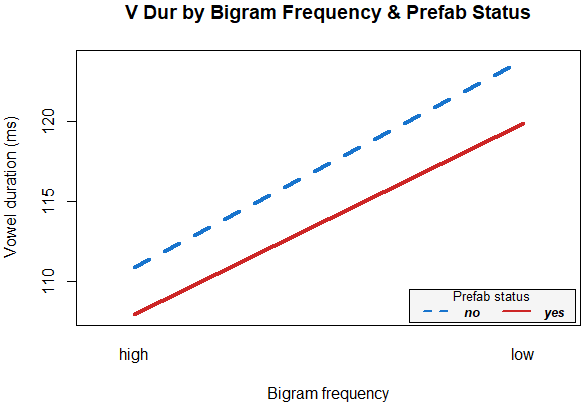
\includegraphics[width=4.2516in,height=2.6709in,width=\textwidth]{bybee-img001.png}

\end{center}
\begin{styleStandard}
\textit{Figure 2: Vowel duration (raw values in ms) given prefab status and bigram frequency score distribution. Prefab data represented by the red line; free AN pairings represented by the dotted blue line. }
\end{styleStandard}

\begin{styleStandard}
Figure 2 suggests that the phonetic effects of prefab status may indeed be independent of bigram frequency scores, with the greatest difference occurring between low-frequency prefabs and low-frequency free AN pairings (top right). Even though this difference in duration failed to reach statistical significance, the trends in the distribution of the data warranted further exploration. 
\end{styleStandard}

\begin{styleStandard}
We then analyzed only the 182 low-frequency (i.e. bigram frequency of 20 or lower) AN sequences in an attempt to obtain a more detailed understanding of the differences in Figure 2. Thus, excluding high frequency sequences, we find once again that prefabs are overall shorter (\textit{mean} = 120ms, \textit{StDev} = 44ms ) than free AN pairings (\textit{mean} = 124ms, \textit{StDev} = 51ms), though this difference is not statistically significant. This trend is depicted in Figure 3 below.
\end{styleStandard}

\begin{styleStandard}
[Warning: Draw object ignored]
\end{styleStandard}

\begin{styleStandard}
\textit{Figure 3}\textbf{\textit{:}}\textit{ Vowel duration in low-frequency AN sequences by prefab status. The graphs on the left show raw values in milliseconds; log-transformed values appear on the right. Low-frequency prefabs are shown in yellow; low-frequency free AN pairings shown in gray. }
\end{styleStandard}

\begin{styleStandard}
The current comparison indicates that the factors that lead to conventionalization of word sequences also play a role in determining the phonetic properties of words and constructions, one which may be independent of frequency (as suggested by Durrant and Doherty 2010). Although more data are necessary to strengthen the current findings, our results indicate that the lexical cohesion found in prefabs may lead to phonetic fusion and reduction in production. A larger number of AN tokens coded for prefab status may reveal that the trends we observed in our small sample in fact show a difference in duration that is statistically significant.
\end{styleStandard}

\begin{listWWNumxxiileveli}
\item 
\begin{stylelsSectioni}
Discussion
\end{stylelsSectioni}

\begin{listWWNumxxiilevelii}
\item 
\begin{stylelsSectionii}
Phonetic indicators of prefab status
\end{stylelsSectionii}
\end{listWWNumxxiilevelii}
\end{listWWNumxxiileveli}
\begin{styleStandard}
The results reported here show that it might be productive to investigate further possible phonetic correlates of conventionalization. The many corpus studies cited in section 1.4 used measures based on frequency and predictability. The phonetic variables investigated were word duration (which included lexical as well as phonetic differences) (Bell et al. 2009, Seyfarth 2014, Sóskuthy \& Hay 2017), t/d deletion in English, vowel reduction and duration (Jurafsky et al. 2001). The more specific reduction processes specific to English—reduction of coronals and vowels—might be good candidates for phonetic features distinguishing prefabs. Our results suggest that vowel duration may be affected by prefab status. Of course, measures based on frequency are more objective and easier to calibrate than a measure based on prefab status, but numerous studies now show that prefab status may be discernible, especially when the data are restricted to a single construction
\end{styleStandard}

\begin{listWWNumxxiileveli}
\item 
\begin{listWWNumxxiilevelii}
\item 
\begin{stylelsSectionii}
Does the adjective predict the noun or the noun predict the adjective?
\end{stylelsSectionii}
\end{listWWNumxxiilevelii}
\end{listWWNumxxiileveli}
\begin{styleStandard}
Coming back to the discussion in section 2 about the directionality of predictability, where we discussed the finding that for English the duration of a word is associated with its predictability from the following word, we can consider with AN sequences what it would mean to say that W2 predicts W1. As mentioned earlier, the studies, such as Bell et al. (2009), that find predictability from the following word is significant in predicting word duration, do not take into account construction type. Their conclusions, therefore, refer only to general processing mechanisms. Our proposal is that truly understanding the predictability data will require examining particular constructions. As AN constructions make up a major portion of bigrams consisting of two content words, they present a good starting point for understanding predictability relations. 
\end{styleStandard}

\begin{styleStandard}
In a AN attributive construction, the noun is considered the ‘head’ syntactically and it also functions as ‘head’ or grounding point semantically. When confronted with an adjective, a language user will not know how to interpret it until the noun is also known, as the abstract meaning of the adjective can only be made concrete when it is applied to a noun. A finding in Öksüz et al. (2020) supports this supposition. They asked L1 and L2 speakers to judge whether English AN bigrams were in common usage or not, and measured their reaction times. High frequency AN bigrams were judged more quickly than low frequency bigrams by both L1 and L2 speakers. In addition, the frequency of the noun affected the reaction time, with faster reactions for high frequency nouns. In contrast, the frequency of the adjective had no effect. These findings suggest that interpreting an AN sequence depends heavily upon accessing the meaning of the noun.
\end{styleStandard}

\begin{styleStandard}
Viewed from another perspective, one could argue that nouns are associated with a restricted range of adjectives. Peppers come in black, white, red, green, yellow, hot, sweet or mild. Wine is red, white, or sparkling. A spectrum is broad or narrow. A while is good, long or short. To some extent it could be argued that the reverse relation also occurs, because \textit{broad }could be said to predict certain nouns, such as \textit{topic, spectrum} or \textit{education.} Nouns selecting adjective may be more common than the reverse, but that has to be a topic for future research
\end{styleStandard}

\begin{listWWNumxxiileveli}
\item 
\begin{stylelsSectioni}
Conclusion
\end{stylelsSectioni}
\end{listWWNumxxiileveli}
\begin{styleStandard}
The current contribution attempts to combine and reconcile quantitative and qualitative analyses, in a search for the factors influencing the properties of words in combination. We argue that predictability measures can be best understood in terms of particular constructions, rather than as general processing mechanisms. Within particular constructions, the relations between words are varied and may depend more on grammatical and functional factors than on frequency of co-occurrence (see Bell \& Plag 2012 for noun-noun sequences). The hypothesis of this chapter is that certain phonetic distinctions, in particular, reduction of vowel duration, corresponds to conventionalization found in lexical prefabs. Our main finding is that prefab status affects vowel duration in adjectives independently of the frequency of the AN bigram. This result suggests that phonetic factors may in the future provide a diagnostic for the elusive notion of conventionality of expression. 
\end{styleStandard}

\begin{styleStandard}
A qualitative assessment of the relation between two content words in sequence is necessary to understanding the role of predictability in processing and storage. An attempt to determine the prefab status of AN bigrams reveals some problems in the criteria proposed in the literature. Examining a set of adjectives from conversation, two important properties of prefabs have emerged: one is that prefabs may be semantically compositional while referring to entities or concepts of some cultural importance and therefore constitute the conventional means of referring to these concepts. The second is that prefabs are not always isolated, but in some cases form clusters of semantically related word sequences. Thus, existing prefabs can be used to spin off new creative combinations demonstrating again how the conventional and the novel form a continuum and interact in language use. 
\end{styleStandard}

\section[References]{References}
\begin{styleStandard}
Bell, Alan, Brenier, Jason M., Gregory, Michelle L., Girand, Cynthia, \& Jurafsky, Dan. 2009. Predictability effects on durations of content and function words in conversational English. \textit{Journal of Memory and Language} 60(1). 92–111.
\end{styleStandard}

\begin{styleStandard}
Bell, Melanie J. \& Ingo Plag. 2012. Informativeness is a determinant of compound stress in English. \textit{Journal of Linguistics} 48. 485–520.
\end{styleStandard}

\begin{styleStandard}
Biber, Douglas, Stig Johansson, Geoffrey Leech, Susan Conrad \& Edward Finegan. 1999. \textit{Longman grammar of spoken and written English}. London: Longman.
\end{styleStandard}

\begin{styleStandard}
Brinton, Laurel J. \& Elizabeth C. Traugott. 2005. \textit{Lexicalization and language change}. Cambridge: Cambridge University Press.
\end{styleStandard}

\begin{styleFooter}
Bybee, Joan. 1998. The emergent lexicon. In Gruber, Katherine M., Kenneth Olson \& Tamra Wysocki (eds), \textit{Papers from the 34}\textit{\textsuperscript{th}}\textit{ Annual Meeting of the Chicago Linguistics Society 2,} 421-435. University of Chicago: Chicago Linguistic Society. 
\end{styleFooter}

\begin{styleStandard}
Bybee, Joan. 2002. Sequentiality as the basis of constituent structure. In Givón, Talmy \& Bertram F. Malle\textit{ }(eds.),\textit{ The Evolution of Language from Pre-Language, }109-134. Amsterdam: John Benjamins.
\end{styleStandard}

\begin{styleStandard}
Bybee, Joan. 2003. Mechanisms of change in grammaticization: the role of frequency. In Janda, Richard \& Brian Joseph (eds.), \textit{Handbook of Historical Linguistics, }602-623\textit{.} Oxford: Blackwell Publishers.
\end{styleStandard}

\begin{styleStandard}
Bybee, Joan. 2010. \textit{Language, Usage and Cognition}. Cambridge: Cambridge University Press.
\end{styleStandard}

\begin{styleStandard}
\textstylegd{Bybee, Joan. 2014. Analytic and holistic processing in the development of constructions. In Arnon, Inbal, Marisa Casillas, Chigusa Kurumada \& Bruno Estigarribia (eds.) \textit{Language in interaction: Studies in honor of Eve V. Clark, }303-313. Amsterdam and Philadelphia: John Benjamins Publishing Co. }
\end{styleStandard}

\begin{styleStandard}
\textstylegd{Bybee, Joan \& Carol Lynn Moder. 2017. }Chunking and changes in compositionality in context. In Hundt, Marianne, Sandra Mollin \& Simone E. Pfenninger (eds.), \textit{The Changing English Language: Psycholinguistic Perspectives, }148-170. Cambridge: Cambridge University Press.
\end{styleStandard}

\begin{styleStandard}
Bybee, Joan \& David Eddington. 2006. A usage-based approach to Spanish verbs of ‘becoming’. \textit{Language }82.323-355.
\end{styleStandard}

\begin{styleStandard}
Bybee, Joan \& Ricardo F. Napoleão de Souza. 2019. Vowel duration in English adjectives in attributive and predicative constructions. \textit{Language and Cognition }11(4).\textstyleDatei{ 555-581.} \textit{doi:10.1017/langcog.2019.32}
\end{styleStandard}

\begin{styleStandard}
Carrol, Gareth \& Kathy Conklin. 2014. Eye-tracking multi-word units: some methodological questions.~\textit{Journal of Eye Movement Research}~\textit{7}(5). 1-11.
\end{styleStandard}

\begin{styleStandard}
Corrigan, Roberta, Edith Moravcsik, Hamid Ouali, \& Kathleen Wheatley. 2009. Introduction: Approaches to the study of formulae.” In Corrigan, R., Edith Moravcsik, Hamid Ouali, \& Kathleen Wheatley (eds.)\textit{ Formulaic Language, Vol 1. Distributiona and historical change, }xi–xxiv. Typological Studies in Language 82. Amsterdam/Philadelphia: John Benjamins.
\end{styleStandard}

\begin{styleStandard}
Croft, William. 2000. \textit{Explaining language change}. Harlow, England: Longman Linguistic Library.
\end{styleStandard}

\begin{styleStandard}
Davies, Mark. 2008–. The Corpus of Contemporary American English: 450 million words, 1990-present. Retrived from {\textless}http://corpus.byu.edu/coca/{\textgreater}.
\end{styleStandard}

\begin{styleStandard}
Durrant, Philip \& Alice Doherty. 2010. Are high-frequency collocations psychologically real? Investigating the thesis of collocational priming. \textit{Corpus Linguistics and Linguistic Theory} 6 (2).125–55.
\end{styleStandard}

\begin{styleStandard}
Ellis, Nick C. 1996. Sequencing in SLA: Phonological memory, chunking and points of order. \textit{Studies in Second Language Acquisition} 18: 91–126.
\end{styleStandard}

\begin{styleStandard}
Ellis Nick C. 2002. Reflections on frequency effects in language processing.~\textit{Studies in Second Language Acquisition}, 24(2): 297-339.
\end{styleStandard}

\begin{styleStandard}
Ellis, Nick C., Rita Simpson-Vlach, and Carson Maynard. 2008. Formulaic language in native and second language speakers: Psycholinguistics, Corpus Linguistics, and TESOL. \textit{TESOL Quarterly} 42 (3): 375–96.
\end{styleStandard}

\begin{styleStandard}
Erman, Britt \& Beatrice Warren. 2000. The Idiom Principle and the Open Choice Principle. \textit{Text} 20: 29–62.
\end{styleStandard}

\begin{styleStandard}
Gardner, Michael K., Ernst Z. Rothkopf, Richard Lapan \& Toby Lafferty. 1987. The word frequency effect in lexical decision: Finding a frequency-based component. \textit{Memory \& Cognition} 15(1)\textbf{, }24–28. https://doi.org/10.3758/BF03197709
\end{styleStandard}

\begin{styleStandard}
Godfrey, John J. \& Edward Holliman. 1993. Switchboard-1 Release 2 LDC97S62. Web Download. Philadelphia: Linguistic Data Consortium.
\end{styleStandard}

\begin{styleStandard}
Gregory, Michelle, L, William D. Raymond, Allan Bell, Eric Fosler-Lussier \& Dan Jurafsky. 1999. The effects of collocational strength and contextual predictability in lexical production. \textit{Chicago Linguistic Society} 35, 151–166.
\end{styleStandard}

\begin{styleStandard}
Gyllstad, Henrik, and Brent Wolter. 2016. Collocational processing in light of the phraseological continuum model: Does semantic transparency matter?~\textit{Language Learning,}~66(2): 296-323.
\end{styleStandard}

\begin{styleStandard}
Haiman, John. 1994. Ritualization and the development of language. In Pagliuca, William\textit{ }(ed.),\textit{ Perspectives on Grammaticalization}, 3–28. Amsterdam: John Benjamins.
\end{styleStandard}

\begin{styleStandard}
Church, Kenneth \& Patrick Hanks. 1990. Word association norms, mutual information, and lexicography. \textit{Computational linguistics} 16(1), 22-29.
\end{styleStandard}

\begin{styleStandard}
Hirst, Daniel J. 1983. Structures and categories in prosodic representation. In Cutler, Anne \& D. Robert Ladd (eds.), \textit{Prosody: models and measurement, }93-110. Berlin: Springer Verlag.
\end{styleStandard}

\begin{styleStandard}
Hoffman, Sebastian. 2004. Are low-frequency complex prepositions grammaticalized? On the limits of corpus data - and the importance of intuition. In Lindquist, Hans \& Christian Mair (eds.),\textit{ Corpus approaches to grammaticalization in English}, 171–210. Amsterdam: John Benjamins.
\end{styleStandard}

\begin{styleStandard}
Jones, Susan \& John Sinclair. 1974. English lexical collocations: A study in computational linguistics. \textit{Cahiers de Lexicologie} 24: 15-61.
\end{styleStandard}

\begin{styleStandard}
Jurafsky, Dan, Alan Bell, Michelle Gregory \& William D Raymond. 2001. Probabilistic relations between words: Evidence from reduction in lexical production. In Bybee, Joan \& Paul Hopper (eds.)\textit{, Frequency and the Emergence of Linguistic Structure}, 229–254. Amsterdam: John Benjamins.
\end{styleStandard}

\begin{styleStandard}
Langacker, Ronald W. \textit{Cognitive grammar: A basic introduction}. Oxford: Oxford University Press, 2008.
\end{styleStandard}

\begin{styleStandard}
Lindblom, Björn. 1990. Explaining phonetic variation: A sketch of the H\&H Theory. In Hardcastle, William J. \& Alain Marchal (eds.)\textit{, Speech production and speech modelling}, 403–39. Dordrecht: Kluwer Academic Publishers.
\end{styleStandard}

\begin{styleStandard}
Matsuki, Kazunaga, Victor Kuperman \& Julie A. van Dyke. 2016. The Random Forests statistical technique: an examination of its value for the study of reading. \textit{Scientific Studies of Reading} 20(1), 20–33.
\end{styleStandard}

\begin{styleStandard}
Morrill, Tuuli. 2011. Acoustic correlates of stress in English Adjective-Noun compounds. \textit{Language and Speech} 55(2). 167–201.
\end{styleStandard}

\begin{styleStandard}
Öksüz, Doğuş, Vaclav Brezina \& Patrick Rebuschat. \ 2020. Collocational processing in L1 and L2: The effects of word frequency, collocational frequency, and association. \textit{Language Learning. }
\end{styleStandard}

\begin{styleStandard}
Oxford Collocations Dictionary (2002). Oxford: Oxford University Press.
\end{styleStandard}

\begin{styleStandard}
Pawley, Andrew. 1986. Lexicalization. In Tannen, Deborah \& James E. Alatis (eds.) \textit{Languages and linguistics: the interdependence of theory, data and application}, 98–120. Washington, D.C.: Georgetown University Press.
\end{styleStandard}

\begin{styleStandard}
Pawley, Andrew \& Frances H. Syder. 1983. Two puzzles for linguistic theory: nativelike selection and nativelike fluency. In Richards, Jack C. \& Richard W. Schmidt (eds.)\textit{, Language and communication}, 191–226. London: Longmans.
\end{styleStandard}

\begin{styleStandard}
Pitt, Mark A., Laura Dilley, Keith Johnson, Scott Kiesling, William Raymond, Elizabeth Hume \& Eric Fosler-Lussier. 2007. \textit{Buckeye Corpus of Conversational Speech (2nd release)} [www.buckeyecorpus.osu.edu]. Columbus: Ohio State University.
\end{styleStandard}

\begin{styleStandard}
R Core Team 2013. R: a language and environment for statistical computing. R Foundation for Statistical Computing, Vienna, Austria. Retrieved from {\textless}https://www.R-project.org/{\textgreater}
\end{styleStandard}

\begin{styleStandard}
Scarborough, Don L., Charles Cortese \& Hollis S. Scarborough. 1977. Frequency and repetition effects in lexical memory. \emph{Journal of Experimental Psychology: Human Perception and Performance, 3}(1), 1–17. \href{https://psycnet-apa-org.libproxy.unm.edu/doi/10.1037/0096-1523.3.1.1}{\textstyleInternetlink{https://doi-org.libproxy.unm.edu/10.1037/0096-1523.3.1.1}}
\end{styleStandard}

\begin{styleStandard}
Schmid, Hans-Jörg. 2017. A framework for understanding linguistic entrenchment and its psychological foundations. In Schmid, Hans-Jörg (ed.)\textit{ Entrenchment and the psychology of language}, 9–35. (Language and the human lifespan). Berlin: Walter de Gruyter.
\end{styleStandard}

\begin{styleStandard}
Seyfarth, Scott. 2014. Word informativity influences acoustic duration: Effects of contextual predictability on lexical representation. \textit{Cognition} 133. 140–155.
\end{styleStandard}

\begin{styleStandard}
Sinclair, John. 1991\textit{. Corpus, Concordance and Collocation}. Oxford: Oxford University Press.
\end{styleStandard}

\begin{styleStandard}
Siyanova-Chanturia, Anna \& Ron Martinez. 2015. The idiom principle revisited.~\textit{Applied Linguistics}~36(5), 549-569.
\end{styleStandard}

\begin{styleStandard}
Sóskuthy, Márton, \& Hay, Jennifer. 2017. \ Changing word usage predicts changing word durations in New Zealand English. \textit{Cognition} 166: 298–313.
\end{styleStandard}

\begin{styleStandard}
Tagliamonte, Sali A. \& Harold R. Baayen. 2012. Models, forests, and trees of York English: was/were variation as a case study for statistical practice. \textit{Language Variation and Change }24(2), 135–178.
\end{styleStandard}

\begin{styleStandard}
Van Lancker, Diana \& Gerald J. Canter. 1981. Idiomatic versus literal interpretations of ditropically ambiguous sentences. \textit{Journal of speech and hearing research} 24. 64–69.
\end{styleStandard}

\begin{styleStandard}
Vilkait\.e, Laura. 2016. Are nonadjacent collocations processed faster?~\textit{Journal of Experimental Psychology: Learning, Memory, and Cognition}~42 (10), 1632-1642.
\end{styleStandard}

\begin{styleStandard}
Wilson, Damián V. 2009. From ‘remaining’ to ‘becoming’ in Spanish: The role of prefabs in the development of the construction \textit{quedar(se)} + ADJECTIVE.” In Roberta Corrigan, Edith Moravcsik, Hamid Ouali, and Kathleen Wheatley (Eds.)\textit{ Formulaic Language}, I:273–95. (Typological Studies in Language 82). Amsterdam: John Benjamins.
\end{styleStandard}

\begin{styleStandard}
Wolter, Brent \& Junko Yamashita. 2018. Word frequency, collocational frequency, L1 congruency, and proficiency in L2 collocational processing: What accounts for L2 performance?~\textit{Studies in Second Language Acquisition}~40(2): 395-416.
\end{styleStandard}

\begin{styleStandard}
Wray, Alison. 2002. \textit{Formulaic language and the lexicon}. Cambridge: Cambridge University Press.
\end{styleStandard}

\section[Appendix 1]{Appendix 1}
\begin{styleStandard}
Adjective-noun sequences classified as prefabs
\end{styleStandard}

\begin{flushleft}
\tablefirsthead{}
\tablehead{}
\tabletail{}
\tablelasttail{}
\begin{supertabular}{m{1.0427599in}m{3.5163598in}}
Adjective &
Noun(s)\\\hline
bad &
\textit{shape, way}\\
broad &
\textit{topic, question, shoulders, background, scope, subject, range, spectrum, humor, daylight, views, coverage, sense, term, education, category, tastes}\\
dead &
\textit{week, body, zone, bodies, wood, period, place}\\
fat &
\textit{wallet, dude}\\
good &
\textit{bit, deal, money, size, behavior, while, buys, condition, shape, portion}\\
hot &
\textit{check, shower, water, topic, fudge}\\
mad &
\textit{rush, dog}\\
red &
\textit{kidney beans, meat, herring, wine, meat, flag, eyes, threat, carpet, alert, lobsters, China, beans, light, snappers, pepper, spider}\\
sad &
\textit{statement, way, commentary}\\
wet &
\textit{labs, rag, rags}\\\hline
\end{supertabular}
\end{flushleft}
\clearpage\setcounter{page}{1}\section[Appendix 2]{Appendix 2}
\begin{styleStandard}
Adjective-noun sequences classified as free combinations
\end{styleStandard}

\begin{flushleft}
\tablefirsthead{}
\tablehead{}
\tabletail{}
\tablelasttail{}
\begin{supertabular}{m{1.0427599in}m{3.5163598in}}
Adjective &
Nouns\\\hline
bad &
\textit{test, types, news, stuff, aspects, experience, thing, speller, cholesterol, team, mayor, points, things, example, weather, habits, signs, sides, knees, influence, meal, habit}\\
broad &
\textit{one, disparities, section, overstatements, word, interest, way, definition, segment, strengths, issue}\\
dead &
\textit{bride, cat, doctors, Iraqi, sport, birds, presidents, poets, shrubs, cat, people, cell phone, protein}\\
fat &
\textit{lady, women, intern, kid, American, Americans, dog, burger, people, kind, man, person, one, ones, kids, boy, cat, days}\\
good &
\textit{trees, movie, area, impact, shows, team, lunch, retirement, movies, idea, information, state, company, French fries, ones, nursing home, summer, ones, question, lesson, way, program, balance, reputation, job, experiences, point, player, weather, weekend, loan}\\
hot &
\textit{events, foods, jacuzzis, summertime, days, things, ones, weather, points, one, water, air, afternoons}\\
mad &
\textit{one}\\
red &
\textit{hat, dirt, insect, suspenders, dress, cat, Doberman, berries, sign, one, dye, ones, streak, house, strips, clay, salmon, Ferrari, badge, day, felt, face, star, birds, house, lightning, shirt, rats, fescue, azaleas, }\\
sad &
\textit{part, thing, things, joke, year }\\
wet &
\textit{cold, dry, food, kind, part, weather, stuff, cloth, June, hair, feed, heat, backyard, mess, towel, sponge, springs, paper towel}\\\hline
\end{supertabular}
\end{flushleft}
\begin{stylelsTranslation}
~
\end{stylelsTranslation}

\clearpage
\end{document}
